\documentclass[12pt, letterpaper, twoside]{article}
\usepackage[utf8]{inputenc}
\usepackage[T1]{fontenc}
\usepackage[polish]{babel}
\usepackage{indentfirst}
\usepackage{enumerate}
\usepackage{graphicx}

\graphicspath{{C:/Users/hubkn/Desktop/Latex/}}

\title{\Huge{\textbf{Platformy Programowania}}}
\author{Hubert Knioła \thanks{Poznań University of Technology}}
\date{\textit{19.01.2021}}
\frenchspacing

\begin{document}

\begin{titlepage}
\maketitle
\end{titlepage}

\tableofcontents

\newpage
\section{Makbet}
\subsection{Information [Task 3]}
\textbf{[textbf] Macbeth, fully The Tragedy of Macbeth,} 
\newline
\texttt{[texttt] is a tragedy by William Shakespeare.}
\newline
\emph{[emph] It was probably first performed in 1606.}
\newline
\textit{[textit] It was first published in the Folio of 1623,}
\newline
\textsc{[textsc] possibly from a prompt book, and is Shakespeare's.}
\newline
\textnormal{[textnormal] James VI and I  was  patron of Shakespeare's playing company,}
\newline
and some people [Task 6] \ref{fig:photo} say [Task 6] \pageref{tab:1} that Macbeth is the play which most clearly indicates Shakespeare's relationship with him. In the play, Macbeth is a Scottish general under the rule of King Duncan. Three witches tell Macbeth that he will become king of Scotland. Macbeth is spurred by his ambition and his wife, murdering Duncan and acceding to the throne. His reign is bloody and tyrannical and is ended by the combined forces of Scotland and England.
\newline
Shakespeare's [Task 8] \cite{firstbib} source  [Task 8] \cite{secondbib} for the story  [Task 8] \cite{thirdbib} was Holinshed's Chronicles, particularly its accounts of Macbeth and Macduff and Duncan, but events in the play differ extensively from events involving the historical Macbeth.[citation needed] Events in Shakespeare's play are usually associated with Henry Garnet and the Gunpowder Plot of 1605. In theatre, the play has been associated with a curse. People have avoided speaking its title, calling it "The Scottish Play": however, the play has attracted some of the most renowned actors to the leading roles and has been adapted for multifarious other media. It has been continuously in production since the 1660s.

\paragraph{Makbet's family}
\ldots
\subparagraph{Makbet's childrens}
\ldots
\subsubsection{Detailed information}
%\ldots

\newpage
\subsection{Other [Task 4]}
\begin{enumerate}[a)]
    \item Egzamin Bazy Danych
\begin{enumerate}[I.]
    \item Python
    \item Java
    \item C++
    \item Prolog
    \item Erlang
    
\end{enumerate}

    \item Egzamin Podstawy Ochrony Danych
    \item Egzamin Grafika
    \item \ldots

\end{enumerate}

\subsection{More [Task 5]}
„I am your father, Anakin Skywalker"
\footnote{I - ja}
\newline
``I am your father, Anakin Skywalker''
\footnote{am - jestem}
\newline
''I am your father, Anakin Skywalker"
\footnote{your - twój}
\newline
`I am your father, Anakin Skywalker'
\footnote{Father - ojciec}
\newline
"I am your father, Anakin Skywalker"

\subsection{More than more [Task 6]}
\begin{figure}[h!]
    \centering
    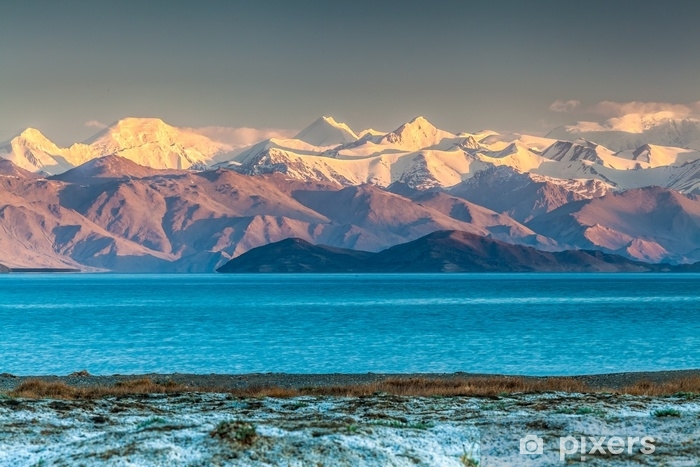
\includegraphics[scale=0.2]{photo}
    \caption{Opis zdjęcia}
    \label{fig:photo}
\end{figure}

\label{tab:1}
\begin{center}
    \begin{tabular}{|c c c c|}    
    \hline
    Województwo & Powierzchnia[km2] & Populacja \\
    \hline\hline
    Mazowieckie & 35 558 & 5 349 114 \\ 
    \hline
    Wielkopolskie & 29 826 & 3 475 323 \\
    \hline
    Lubelskie & 25 122 & 2 139 726 \\
    \hline
   \end{tabular}
\end{center}

%\large{[Task 6] \ref{fig:photo}}
%\newline
%\large{[Task 6] \pageref{tab:1}}

\subsection{Mathematics [Task 7]}
\begin{enumerate}[a)]
    \item \( {n \choose k} = \frac{ n! }{ k!{n-k}! }\)
    \item \( a^{2} + b^{2} = c^{2}\)
    \item \( \frac{\frac{1}{2} + \frac{1}{4}}{\frac{1}{8}} \neq 1\)
    \item \( \sum_{i=1}^{n} i^{2} = \frac{n(n+1)(2n+1)}{6}\)
    \item \( C_{2}^{-3} + O_{2}^{0} \rightarrow C_{}^{+4}O_{2}^{-2} + H_{2}^{+1}O_{}^{-2}\)
    \item $$\mathbf{X} =
    \left( \begin{array}{cccc}
    a_{1,1} & a_{1,2} & \ldots &a_{1,n} \\
    a_{2,1} & a_{2,2} & \ldots &a_{2,n} \\
    \vdots & \vdots & \ddots & \vdots \\
    a_{m,1} & a_{m,2} & \ldots & a_{m,n}
    \end{array} \right)$$
\end{enumerate}

\section{Romeo and Julia [Task 8]}

\bibliographystyle{unsrt}
\bibliography{bible}

\end{document}